\chapter{Evaluation}

In this chapter, experiments are conducted in order to evaluate the application based on the system requirements defined in the problem statement: 

\begin{enumerate}
    \item The application should provide an interface for the patient to 1) record physiological signals (e.g., during sleep); 2) present the results; and 3) share the results.
    \item The application should provide an interface for the developers to create modules to enrich the data from records or extend the functionality of the application. 
    \item The application should ensure a seamless and continuous data stream, uninterrupted from sensor disconnections and human disruptions.
\end{enumerate}

The experiments are designed to test the application in (A) a crowded environment with multiple Flow sensors and without different Android OS versions; (B) recording over an extended period to measure battery consumption; (C) user-friendliness on participants; and (D) creating a simple module. When evaluating the experiments, the observations and the results are the most interesting metric as it provides a better perception of whether the design choices (Chapter 4) and implementation (Chapter 5) suffice towards the goal of this thesis. Moreover, the observations and results allow for discussion on improvements which can be made in future work.  


\section{Experiment A: Orchestral Concert to Analyze Musical Absorption using Nidra to Collect Breathing Data}
This experiment was conducted in collaboration with master student Joachim Dalgard at the University of Oslo at \textit{RITMO: Centre for Interdisciplinary Studies in Rhythm, Time and Motion}. 

The goal of the experiment for Dalgard was to analyze musical absorption, which is a state when individuals allow music to draw them into an emotional experience and becomes unaware of time and space. In order to analyze the effect of musical absorption on individuals, Dalgard gathered 20 participants who were experienced listeners with musical education. The participants attended an orchestral concert by Richard Strauss' Alpine Symphony---a symphonic poem that portrays the experience of eleven hours spent climbing an Alpine mountain---that lasted approximately 50 minutes at Oslo Concert Hall on April 3rd and April 4th, 2019.  

With respect to Nidra, the motivation for this experiment can be summarized into: (1) to test the application in a real-life and crowded environment, in order to analyze whether other mobile devices interfere or obstruct with the signals between the collecting sensors and mobile devices; (2) to test whether the samples gathered are meaningful, in the sense that the application is collecting the samples from the sensors correctly and handling unexpected disconnections; and (3) to test the application on different Android OS versions, and to put the application in the hands of participants. 

The participants were divided into two groups to attend the concert on the two dates. Each participant was equipped with a wireless electromyographic sensor from DELSYS in order to measure heart rate, and a Flow sensor to measure respiration during the concert. RITMO had multiple Flow sensors for disposal; however, they had no suitable mobile application that could record data from these sensors. Also, with the equipment they indented to us, they experienced that Flow sensor tended to disconnect every 10-15 minutes resulting in fragmented recordings for a single session. Therefore, they reached out to the \textit{Insitute for Informatics} in hopes of a solution. Our application was a suiting match for both parties, and we could combine the analysis of musical absorbation with the evaluation of Nidra. We arranged for six Android devices and reached out to the participants to bring their Android devices if they had one. Thus, there were ten participants in each group and six assessed devices. As a precaution, we decided to give out the devices to the participants who scored highest on a test performed on beforehand.

During the concert, there were approximately 800 attendees on the first day and approximately 1500 attendees on the second day. We assume that most of the attendees had a mobile device, and probably many of them had BlueTooth activated on the device. As such, we were able to replicate an environment (on a larger scale) where other devices might interfere with the signals between the collecting sensor and the mobile device during recording. Also, we were able to install the application on multiple mobile devices with different Android OS versions and put the application in the hands of the participants. 

\subsection{Preperations}

\begin{table}
\begin{center}
\scalebox{0.59}{
\begin{tabular}{ |c|c|c|c| } 
\hline
\textbf{Model} & \textbf{Samsung Galaxy S9} & \textbf{OnePlus 3T} & \textbf{Google Pixel XL} \\
\hline
Operating System & Android 8.0 & Android 8.1 & Android 9.0 \& Android 7.1.2  \\
\hline
Chipset & Exynos 9810  & Qualcomm MSM8996 Snapdragon 821 & Qualcomm MSM8996 Snapdragon 821  \\
\hline
CPU & Octa-core & Quad-core & Quad-core \\
\hline
GPU & Mali-G72 MP18 & Adreno 530 & Adreno 530  \\
\hline
RAM & 4 GB & 6 GB & 4 GB \\
\hline
Battery & Li-Ion 3000 mAh & Li-Ion 3400 mAh & Li-Ion 3450 mAh  \\
\hline
Bluetooth & 5.0, A2DP, LE, aptX & 4.2, A2DP, aptX HD, LE & 4.2, A2DP, LE, aptX \\

\hline
\end{tabular}}
\caption{Device models used during the concert}
\end{center}
\end{table}

To prepare for the experiments, we configured the applications on the assessed mobile devices and stress-tested the application to prevent any unforeseen events or bugs that could occur during the recording. Also, before the concert, we had to ensure that each participant had the sensors placed correctly on their body and given the right mobile device. Below, we describe the preparation in more detail.

\begin{description}
    \item[Device Configuration] The device models in our disposal had to be configured with the applications to enable recording on Nidra. First, the data stream dispatching module was installed on the devices. Second, the sensor wrapper for the Flow sensor was installed on the devices and configured with one Flow sensor---in order to reduce the time to set up the mobile device with a Flow sensor on the participant before the concert. Lastly, the Nidra application was initiated with the id (A--F) of the sensor that the participant should use to keep track of each participant's sensor and device model. In Table 6.1, the device models are listed with their specifications and Android version. In the following list the id is mapped with the device model; the experiment will describe the device model based on the id, respectively: (A, B, C) Samsung Galaxy S9; (D) Google Pixel XL (version: 9.0); (E) Google Pixel XL (version: 7.1.2); and (F) OnePlus 3T. 
    \item[Body Placement] The respiration (breathing) value is based on the participant body circumference, and changes are associated with breathing. The participant was instructed to place the sensor around their thorax (just below the armpits), in order to measure the expansion and contraction of the rib cage.

\end{description}

\subsection{Results}

The records from the various mobile devices were gathered by using the sharing functionality in the application and sent to our application (over e-mail). There were thirteen mobile devices combined for both dates---one of the participants had an Android device---however, the application crashed on one of the mobile devices during the recording. Therefore, we have access to twelve recordings from the concerts. 

\begin{figure}[!h]
    \centering
    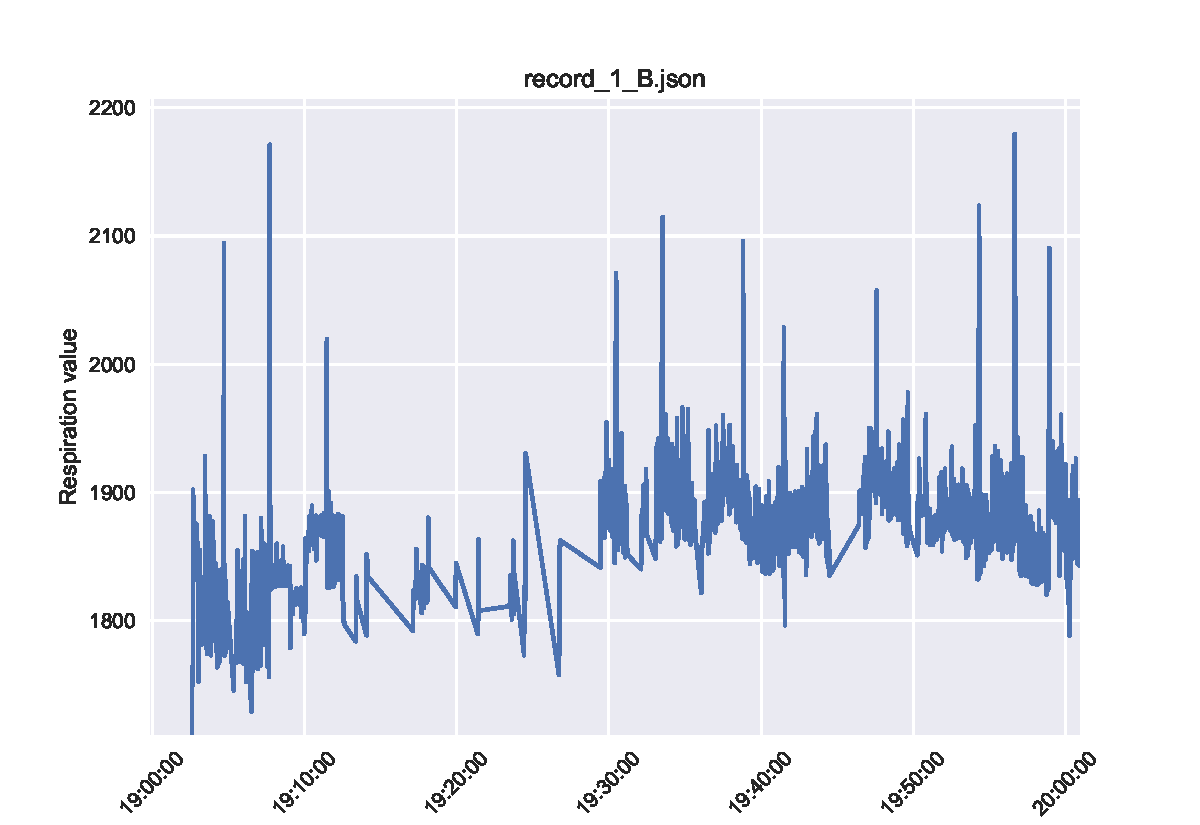
\includegraphics[scale=0.5]{images/Record_1_B.pdf}
    \caption{Implementation of recording functionality (A): start recording}
    \label{fig:day_1}
\end{figure}

\begin{figure}[!h]
    \centering
    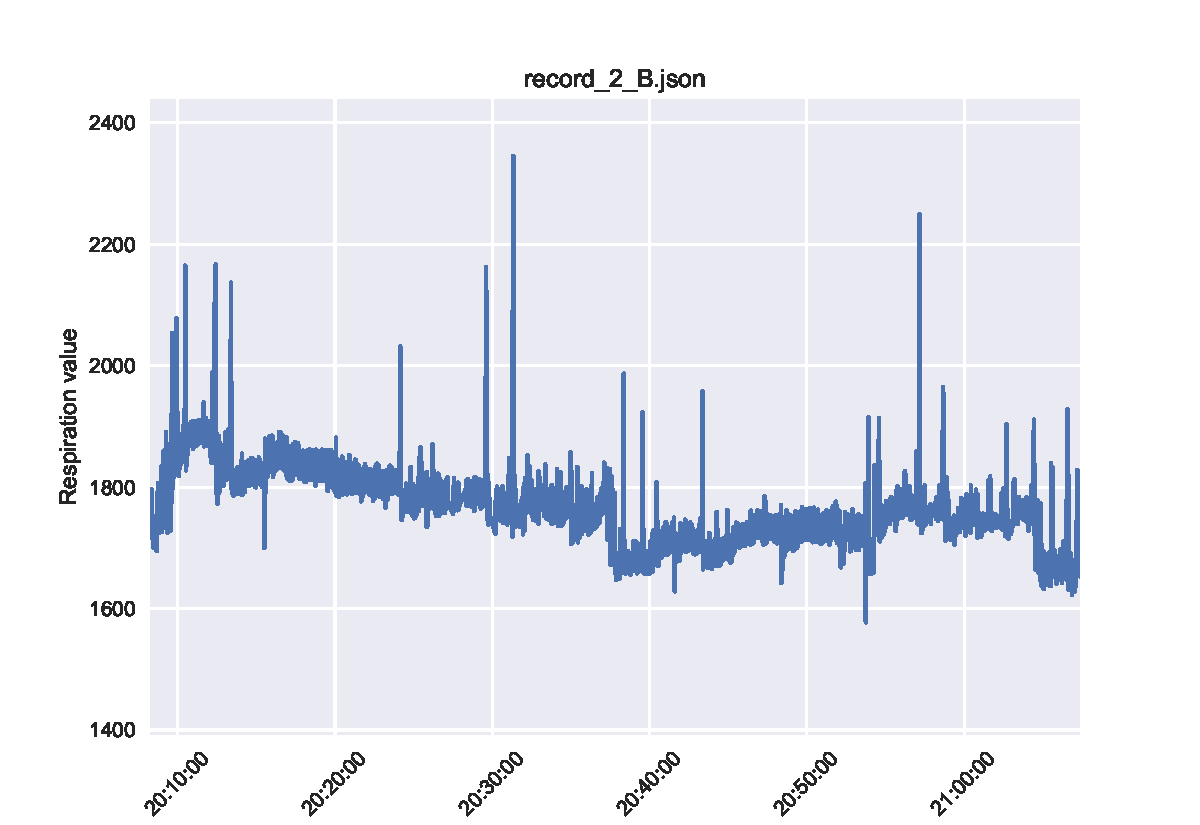
\includegraphics[scale=0.5]{images/Record_2_B.pdf}
    \caption{Implementation of recording functionality (A): start recording}
    \label{fig:day_2}
\end{figure}



Figure \ref{fig:day_1} and Figure \ref{fig:day_2} present two of these twelve recordings (rest can is found in Appendix B) that are of most interest to us in a time-series graph. The Y-axis represents the respiration (breathing) value, and the X-axis the time of respiration value acquisition---\textit{day one} of the concert started at the time of 19:00 and ended at 20:00, while \textit{day two} started at the time of 20:10 and ended 21:00.

Moreover, from the thesis by Løberg \cite{fredrik}, we can group the signals strengths based on four types of breathing patterns: (1) \textit{normal breathing}---normal exhaling and inhaling (12-18 breaths per minute); (2) \textit{no breathing}---close to flat rates over a long period; (3) \textit{shallow breathing}---rapid inhaling and exhaling; and (4) \textit{deep breathing}---prolonged inhaling or exhaling (also denoted as fluctuations). From the figures, we can see that the respiration value is stable with some fluctuations and disconnections. Disconnections are defined as when the line is sloping or benching in an extended period (e.g., 20 seconds or more), while fluctuations are samples that spikes (deep breathing) in the graph. We should keep in mind that the margin for the normal breathing respiration value can vary throughout the recording based on body or sensor position and movements (e.g., sitting relax or tense on a chair). 

Figure 6.1 has many disconnections (further analyzed later) with unstable breathing. There are multiple occurrences of deep breathing throughout the recording, with some shallow breathing at the start and end of the recording. Hypothetically, deep breathing might be a sign of musical absorption; however, we have no concrete analysis of this matter, and it is out of the scope for this experiment motivation. Moving on, Figure 6.2 shows fewer disconnects compared to Figure 6.1, and with much more concise breathing patterns and resemblance to normal breathing. Although, there are noticeably deep breathing throughout the recording, with a few shallow breathings at the beginning. Conclusively, both Figures shows no signs for no breathing during the recording. However, there are signs of normal breathing, with few instances of shallow and deep breathing. 

\subsection{Analysis \& Discussion}
In this section, we will discuss all twelve records by analyzing the data. It is of special interest to find occurrences of disconnections---when the samples are stagnant in more extended period---and the time the sensor is disconnected during the recording.

\begin{table}[!h]
\begin{center}
\scalebox{0.7}{
\begin{tabular}{ |c|c|c|c||c|c| } 
\hline
\textbf{Model} & \textbf{Samples Count} & \textbf{Loss Count} & \textbf{Loss Percentage} & \textbf{Disconnection Count} & \textbf{Disconnection Time} \\
\hline
A & 5145 & 0 & 0 \% & 0  & 00:00  \\
\hline
B & 3363 & 1782 & 34 \% & 13 & 19m:14s  \\
\hline
C & 4189 & 956 & 19 \% & 7 & 8m:20s  \\
\hline
D & 3501 & 1644 & 32 \% & 5 & 18m:30s  \\
\hline
E & 5144 & 1 & 0.02 \% & 0 & 00:00  \\
\hline
F & 5145 & 0  & 0 \% & 0 & 00:00  \\
\hline
\end{tabular}}
\caption{Day 1---Duration: 1 hour \& Expected Sample Count: 5145}
\end{center}
\end{table}


\begin{table}[!h]
\begin{center}
\scalebox{0.7}{
\begin{tabular}{ |c|c|c|c||c|c| } 
\hline
\textbf{Model} & \textbf{Samples Count} & \textbf{Loss Count} & \textbf{Loss Percentage} & \textbf{Disconnection Count} & \textbf{Disconnection Time} \\
\hline
A & 4286 & 2 & 0.05 \% & 0  & 00:00  \\
\hline
B & 4161 & 127 & 3 \% & 4 & 1m:25s  \\
\hline
C & 4286 & 2 & 0.05 \% & 0 & 00:00  \\
\hline
D & 2576 & 1712 & 40 \% & 7 & 24m:35s  \\
\hline
E & 4285 & 3 & 0.06 \% & 0 & 00:00  \\
\hline
F & 4288 & 0  & 0 \% & 0 & 00:00  \\
\hline
\end{tabular}}
\caption{Day 2---Duration: 50 mins. \& Expected Sample Count: 4288}
\end{center}
\end{table}

After analyzing the data from the record, Table 6.2 and Table 6.3 presents the six devices for the two dates. Each table exhibits data that is extracted from each recording from the mobile device and can be characterized as: 

\begin{description}
    \item[Expected Sample Count] The expected number of samples that can be acquired in the period of the recording (based on the frequency of sample output by Flow sensor, which is approximately 1.5 Hz).
    \item[Sample Count] The number of samples that were gathered in the duration of the recording. 
    \item[Loss Count] The number of missing samples based on "expected sample count". This can be calculated as: 
\begin{equation} \label{losscount}
Loss\ Count = Expected\ Sample\ Count - Samples\ Count
\end{equation}
    \item[Loss Percentage] The percentage of missing samples based on the expected samples. This can be calculated as:
\begin{equation} \label{losscount}
Loss\ Percentage = (1 - \frac{Samples\ Count}{Expected\ Sample\ Count}) * 100
\end{equation}
    \item[Disconnection Count] Is the number of disconnections that occurred within the duration of the recording.
    \item[Disconnection Time] Is the accumulated time of disconnections. 
\end{description}

The device models A, E, and F are noticeably accurate (with some noises which presumably occurred during parsing); there are no apparent disconnects during the recording for these models both of the days. However, model B and C show a high loss count on the first day---with a disconnection count of 13 of which the disconnection time is 19 minutes and 14 seconds (34\% loss percentage) for model B, and a disconnection count of 7 of which the disconnection time is 8 minutes and 20 seconds (19\% loss percentage) for model C---while on the second day, the loss percentage decreased with 31\% for model B and 18.95\% for model C, resulting in a close to  0\% loss percentage for both devices; noticeably, model B shows four disconnects during the recording, however, they only last for 1 minute and 25 seconds in total. Moreover, device model D shows an alarmingly high loss percentage, which is reflected in the disconnection time, both of the days. The mobile device has a loss percentage of 32\% on the first day and 40\% the second day, that is an increase of 8\% of the day before. 

Based on the analysis, we can see a variety of behavior of disconnections on the mobile devices for the two dates. An assumption is that the mobile device or Flow sensor is malfunctioned; however, we have no data that indicates whether a sensor was connected with the same mobile device for the both dates---we had the data for the first date, however, the sensors and mobile devices were switched at the second date because of unforeseen events---therefore, this assumption is debunked. Moreover, we see that model D (Google Pixel XL, version 9.0) is unstable for both of the days, in contrast to the other device models which ran a lower Android version. However, yet again, we no accurate data that can prove that the Android version, mobile device, or the Flow sensor is causing the disconnects---albeit, this can be further tested in the lab.

\subsection{Conclusion}
To summarize the experiment, we were able to test the application in a real-life and crowded environment. The application managed to record samples that lasted up to 1 hour with the Flow senor and various device models with different Android OS versions. However, one of the application crashed, and we were unable to find the source of the problem. Based on the samples from the records, it is identified that the Flow sensor has a tendency of disconnecting, but the application managed to reconnect with the sensor during the recording. In the end, the records were successfully shared across applications, which enabled us to analyze the recordings.  

To conclude, we will evaluate whether the tests sufficed the motivation of the experiement:

\begin{enumerate}
    \item \textit{test the application in a real-life and crowded environment, in order to analyze whether other mobile devices interfere or obstruct with the signals between the collecting sensors and mobile devices.}
    
    While we are able to conduct an experiment which had approximately 800 attendees on the first day and approximately 1500 attendees on the second day of which probably most had their BlueTooth activated, the experiments lack data to support that the interference did affect the sampling from the Flow sensor to a mobile device. However, all of the recordings show at least 60\% of the concert was recorded (and some recordings are 100\%). To conclude this test, there is insufficient data to show for inference affected the recording; however, were are able to test the application in a real-life and crowded environment. 

    \item \textit{test whether the samples gathered are meaningful, in the sense that the application is collecting the samples from the sensors correctly and handling unexpected disconnections.}
    
    As discussed in the analytics section, model device A, E, and F were able to collect data throughout the concert for both days. Model B, C, D had disconnects during the recording; however, all managed to reconnect during the recording. As a result, no more than 40\% of the recording was lost for both of the days. To conclude this test, the application can successfully reconnect with the connected Flow sensor during the recording, which results in the data is more meaningful for further analysis. 

    \item \textit{test the application on different Android OS versions, and to put the application in the hands of participants.} 
    
    We had a wide variety of device models with different Android OS versions running the application (Nidra). To conclude this test, the application was able to run all of the Android version, regardless of the device model, successfully. Also, we were able to put the application in the hands of other participants that used the application in order to measure their breathing data during the concert.

    As a side note, a questionnaire was sent to the participants in order to get feedback on the user-friendliness of the application; however, none of them took the time to answer the questions.


\end{enumerate}


\section{Experiment B: 9-Hours Recording}
As part of this thesis is to collect breathing data over en extended period (e.g., during sleep), it is essential to test for battery usage during this period. In most cases, a user connects their device to a power source to charge the device battery. However, in the cases where that is not viable, the battery consumption of the applications might affect the perception of the application to the user. Therefore, in this experiment we are checking for the battery consumption on the mobile device, as well as the Flow sensor, to demonstrate that the application is suited for collecting data overnight.

\subsection{Description}
The experiment was conducted on OnePlus 3T device (specifications in Table 6.1), and we started of by configuring the Flow sensor wrapper to connect with the Flow sensor and pressing the "record" button in Nidra. The device and sensor started with 100\%. Also, the device was disconnected from WiFi and left stationary and unattended during the period of recording.  

A technical description of collecting, the data from the Flow sensor and the Nidra is that the Flow sensor collects data on 10Hz; however, it sends a packet of data at approximately 1.5 Hz. The data packet is processed by the Flow sensor wrapper and sent to the data stream dispatching module (DSDM). The DSDM has a list of subscribing applications, and distribute the data packet to all of the subscribing application. In our case, the Nidra application has subscribed for the Flow sensor packets. In Nidra, the packet is received, unpacked and immediately stored in a database as a sample entity, with an identifier of the recording session. This process continues until the recording has terminated based on the user's actions.

\subsection{Results}

We calculate the energy consumption---which is measured in milliampere-hour (mAh)---and estimate the average energy consumption during the experiment. 
\begin{equation} \label{losscount}
Battery\ Consumption = \frac{(start\% - end\%) * device\ capacity\ (mAh)}{recording\ duration\ (hours)}
\end{equation}
Based on the difference of start mAh and end mAh, multiplied by the device battery capacity and divided by the duration of recording, the energy consumption per hour is calculated. 

The application collected 45468 samples from the Flow sensor over the course of 9 hours. That means, the sensor sent data packets on a frequency of approximately 1.5 Hz, which is accurate with previous tests. The mobile device had a battery level of \textit{59\%}, and the Flow sensor had a battery level of \textit{94\%} at the end of the recording. Using Equation \ref{losscount}, we can calculate the average mAh consumed during 9 hours of recording. 
\begin{equation}
\frac{0.41 * 3400}{9} = 154.89\ mAh
\end{equation}
As a result, the device uses approximately 155 mAh. This means that the total battery consumption over the course of the recording was 1395 mAh. Moreover, the device could have been continuing recording for approximately 13 hours more, before running out of battery. Keeping in consideration that the mobile device has an average battery capacity, with a degraded battery capacity due to age, the results seem adequate. However, to compare the results with another application with the same criteria (the same device that is stationary with WiFi turned off), we tested the Spotify application---an application for streaming music---by downloading a song and allowing it to play in the background.
\begin{equation}
\frac{0.025 * 3400}{1} = 85\ mAh
\end{equation}
Using Equation 6.3, we have a rough estimate of the battery usage for the Spotify application. The application drained close to 3\% of the battery percentage during 1 hour of streaming; resulting in an approximately 85 mAh consumption.  

\subsection{Discussion}
The results show that the process of recording consumes close to two times more battery in comparison with listing to music in the background. While the Spotify application plays a downloaded song in the background, the Nidra application operates with two other applications that forward data collected over BlueTooth in the background. As such, the amount of battery consumption is reflected in the process of recording. 

A proposition to reduce the amount of background processing in order to preserve the battery capacity of the mobile device, is to extend the sensor wrapper with a temporary cache or data storage. As such, the data packets are stored in the sensor wrapper during the recording and sent to the subscribing application when the recording is stopped. However, this complicates the structure of a sensor wrapper and might not be feasible in all cases (e.g., the real-time graph becomes obsolete). Although, it can be part of a power-saving configuration in the future. 


\subsection{Conclusion}
To summarize, in this experiment, we used the recording functionality in Nidra. To enable this functionality, Nidra notifies the Flow sensor wrapper through the data streams dispatching module to start the data acquisition. The Flow sensor samples data on a frequency of approximately 1.5Hz and the data are forwarded from the sensor wrapper to the data stream dispatching module, which further distributes the data packets to the subscribed applications. Nidra processes the data packets by unpacking and storing them respectively in the database. At the end of the 9-hours recording, the application collected 45468 samples. As a result, the mobile device used \textit{41\%} of the battery (1395 mAh) and the Flow sensor used \textit{6\%}. Moreover, the device had the possibility of recording for an extra 13 hours.

To conclude, the results of the experiments show that the requirements for recording over an extended period are satisfied. The application can collect data from the Flow sensor, and it is sufficient enough to do it for an extended period. The energy consumption might seem high; however, that is reflected by three applications running simultaneously in the background and data being collected over BlueTooth. Nonetheless, the experiment was successfully conducted, with no apparent form for disconnects or abruptions during the recording. 

\section{Experiment C: Performing User-Tests}
One goal of this thesis is that it should be user-friendly for patients to use and understand the functionality of Nidra. To evaluate whether this goal has been achieved, we found two participants that agreed to partake in the experiment. One of these participants was not proficient in the use of modern technology, while the other participant was tech-savvy\footnote{well proficient in the use of modern technology.}. For simplicity, we will refer to the participant as participant \verb|A| and \verb|B|, respectively. 

The process of this experiment consisted of three parts: a presentation of the application; testing the function of recording, sharing, analyzing; and a survey to evaluate the experience. The testing was not performed overnight, as we focus on user-friendliness, rather than recording over an extended period. 

\begin{description}
    \item[Presentation] We described the functionality of the application to the participants simply and intuitively---without showing the application. That included the explanation of the recording functionality, possibilities of viewing the data in a graph, and the methods of sharing the recording across applications. The presentation took approximately 10 minutes, including questions and clarifications.  
    \item[Tests] The tests were mainly designed to evaluate \textit{comprehensibility} and \textit{usability} in the application. Comprehensibility is to evaluate the participants' ability to understand the functionality of the application, while usability to measure ease of use of the application.
    \item[Survey] The participants were instructed to fill out a questionnaire after these tests were conducted---such that the participant had their feedback fresh in memory. We structured the questions in the questionnaire accordingly to the PACMAD methodology. 
\end{description}

\subsection{Testing}
To evaluate whether the application presents the functionality adequately and suffice the goal of the tests, we tested the participants with certain tasks:
\begin{itemize}
    \item[T1] Proceed to navigate in the application and start a recording.
    \item[T2] Find the interface to view statistics in order to check for connected sensor sources and the graph for the sampling.
    \item[T3] Stop the recording and give the record a name, description, and rating.
    \item[T4] Find the record in the feed of recordings. 
    \item[T5] Share the record over e-email.
    \item[T6] View the analytics for the record and interacting with the graph (e.g., zooming and scrolling). 
\end{itemize}

For this test to be successful, the participants must for all of the tasks be able to identify the actions correctly. These tests were designed to observe the process of recording, sharing, and analyzing. Thus, the functionality of modules were left behind. 


\subsection{Observations}
Participants \verb|A|---less technical---had to familiarize with the setting of the application, thus had a hard start. It took the participant longer than expected to perform T1, however, managed to proceed on the recording. The participant was a bit uncertain whether the recording had started or not. However, the participant was flabbergasted by the rippling effect the recording screen presented. The T2 was somewhat tedious to perform because the participant tried to click on the interface where it says it should be expanded (by swiping). Also, the graph was a bit hard to interact with because the interface above the graph kept moving while performing interactions with the graph. T3 and T4 went fine, the participant filled out the title, description, and a rating and saved the recording, and found the recording on the feed screen. However, T5 and T6 were a bit unclear to the participant, because the records in the list are collaped, and in order to find the actions you have to press the record to expand the information. However, after that figuring out how to expand the records, the participant managed to perform both tasks sufficiently.

Participants \verb|B| outperformed participant \verb|A|, due to the participant was more familiar with technical systems. The participant managed to start the recording quickly, however, was unsure whether the recording had started (clicking around on the interface for feedback) until the ripple effects appeared on the screen. Similar to participant A, participant B clicked on the interface for statistics, rather than swiping, and had a hard time to interact with the graph due to the interface moving. The participant B managed to perform T3-T6 with ease and without any interrupts or objections. 

\subsection{Survey}
A questionnaire was filled out by the patients after the tests. The questions followed a PACMAD survey structure, which is a model to identify the usability attributes and are structured into: effectiveness, efficiency, satisfaction, learnability, memorability, errors, and cognitive load. We created a survey based on some of the structure; however, we were unable to perform any cognitive load or memorability tasks during the testing. Hence, the participant filled out the questions regarding---where 1 is very-hard/very-bad/not-satisfied, and 5 is very-good/very-easy/very-satisfied: 

\noindent \textbf{Effectiveness \& Efficency}
\begin{itemize}
    \item What were your initial thoughts on the application
    
    \begin{description}[font=\normalfont\itshape]
        \item[Participent A:] It looked nice and simple.
        \item[Participent B:] The application seemed very modern and elegant.  
    \end{description}
    
    \item How difficult was it to start a recording
    
    \begin{description}[font=\normalfont\itshape]
        \item[Participent A:] 3
        \item[Participent B:] 4
    \end{description}

    \item How would you rate the feedback you got during a recording 
    \begin{description}[font=\normalfont\itshape]
        \item[Participent A:] 2
        \item[Participent B:] 3
    \end{description}

    \item How difficult was it to stop a recording?
    \begin{description}[font=\normalfont\itshape] 
        \item[Participent A:] 5
        \item[Participent B:] 5
    \end{description}
    \item How difficult was to browse/find previous recordings? 
    \begin{description}[font=\normalfont\itshape]
        \item[Participent A:] 3
        \item[Participent B:] 5
    \end{description}
    \item Did you have any encounters were the application did not supply you with enough information?
    \begin{description}[font=\normalfont\itshape]
        \item[Participent A:] On the recording screen. 
        \item[Participent B:] The recording screen could have been more informing, with more text or an introduction of how the process of recording works. Besides this, everything worked fine.
    \end{description}
\end{itemize}

\noindent \textbf{Satisfaction}

\begin{itemize}
    \item How satisfied were you with the "journey"?
    \begin{description}[font=\normalfont\itshape]
        \item[Participent A:] 4
        \item[Participent B:] 4
    \end{description}
    \item How satisfied were you with this application overall?
    \begin{description}[font=\normalfont\itshape]
        \item[Participent A:] 5
        \item[Participent B:] 4 
    \end{description}
\end{itemize}

\noindent \textbf{Errors}

\begin{itemize}
    \item If you encountered any crashes or errors during the time you used the application, please answer the question below.
    \begin{description}[font=\normalfont\itshape]
        \item[Participent A:] None.
        \item[Participent B:] None.
    \end{description}

\end{itemize}

\noindent \textbf{Feedback and Improvements}

\begin{itemize}
    \item How user friendly did you find the application to be? 
    \begin{description}[font=\normalfont\itshape]
        \item[Participent A:] 4
        \item[Participent B:] 4
    \end{description}
    \item How would you rate the color palette of the application? 
    \begin{description}[font=\normalfont\itshape]
        \item[Participent A:] 5
        \item[Participent B:] 5
    \end{description}
    \item How would you rate the general layout of the application (buttons, text, navigation, etc...)?
    \begin{description}[font=\normalfont\itshape]
        \item[Participent A:] 5
        \item[Participent B:] 5
    \end{description}
    \item Do you have any feedback/improvements to the application itself?
    \begin{description}[font=\normalfont\itshape]
        \item[Participent A:] No.
        \item[Participent B:] Nothing more than I described earlier.
    \end{description}
\end{itemize}

\subsection{Discussion}

As for the observations, the participant managed to perform most of the tasks, albeit the task T1 and T2 were hard to comprehend. Both participants had difficulties in understanding whether the sensor was collecting data, despite the ripple-effects on the screen. The source of this problem is that the sensor some times takes up to 30-60 seconds to start collecting data, making the user wait on the ripple-effect that indicates that the recording has started. Arguably, the user can familiarise with the state of the recording and the ripple-effects; however, to a new user that is not feasible. Also, the interface for statistics was a bit tedious to work with, mainly due to the swiping effect to show the interface and the interactions with the graph making the interface move. Besides this, there were no noticeable complains by the participant. 

As for the survey, the observations reflect the answers in the questionnaire. Most of the poor feedback was directed towards the recording screen being less informative than expected. They found the color scheme of the application to be smooth and fitting, and the application to be modern. Also, they found the general layout to be well organized and overall the application to be user-friendly.


\subsection{Conlusion}

To summarize, we conducted an experiment on two participants with a predefined set of tasks in order to measure the user-friendliness of the application (Nidra). Most of the tasks were regarding the functionality of recording, sharing, and analyzing. The participants were presented with a brief overview of the functionality of the application before starting the testing. The tests were mainly designed to evaluate the comprehensibility and usability of the application. During the testing, we observed the interactions the participants made for each task and followed up with a survey for them to answer. Based on this, we gained a broader understanding of the user-friendliness of the application.

To conclude, the tests were created to measure the comprehensibility and the useability. Overall, the application suffices these measurements; however, the recording screen can be improved in the future. In our perspective, the amount of action that can be performed in that particular screen is limited to three actions (e.g., starting the screen, viewing the statistics, and stopping the recording). However, the participants were not familiarized with the setting of the recording functionality, in which we could have introduced the functionality of the recording even further (e.g., with more text or an introduction before the recording screen). Besides this functionality, the participants found the rest of the application to be pleasant. Noteworthy, the user is restricted to perform the maximum of three actions per screen, in order to reduce the number of actions that can be performed on a screen and for the simplicity of the application. 

To have extended this experiment, we could have invoked tests to measure the cognitive load and memorability of the application. As such, we could have determined whether the application is too tedious to use in the longer run. However, the lack of participants made it hard to evaluate the user-friendliness of the application in the long run.

\section{Experiment D: Creating a Simple Module}
One of the requirements in this thesis is to provide an interface for the developers to create modules, which allows for data enrichment and extended functionality. In order to test for this, we found one participant that had experience in software development, and with some experience in Android development.

 The tests consisted of creating a new module that utilizes the records from Nidra, and to find the record with the highest number of samples. Moreover, it was sufficient to display the correct answer on the screen (the development of a user-interface was not evaluated). Based on these tests, we will evaluate the procedure and the difficulties of creating a new module. 

Before the participant started on creating a new module, we introduced the concepts and data structure of Nidra. Mainly, that Nidra formats the all of the data (e.g., records and corresponding samples) into a JSON string, and the JSON string is put into a bundle with the key \textit{data}, and sent upon launch of the module-application. 


\subsection{Observations}
Although the first task seem intuitive, the participant had a rough start. The participant was aware that module-application received data in a bundle, and the data extraction could be performed by specifying the key. However, for each time the participant compiled, the module-application crashed---that is because the bundle is empty if the module-application is launched directly, and not through the Nidra application (which supplies the module with the data). However, that was corrected quite quickly. 

The next challenge for the participant was to understand how to decode the JSON string into valid objects in Java. The participant studied the structure of the string received on the launch and managed to come up with a solution. First, the participant had created an object which encapsulates the record and a list of samples. Then, three separate objects (i.e., record, sample, and user) had to be created that were identical to the data structure. In the end, the participant could decode the JSON string into a list and retrieve the necessary data.

Once the participant had all of the data, the final task was easily accomplished. The participant iterated through the list of records, and found the one with the highest sample count, and displayed it on the screen. 

\subsection{Results}

At the time of the experiement, there were five records on the mobile device and the highest was the record named \textit{Record 17} with \textit{163 samples}. The participant's module display the same information. Thus, the experiement was successful conducted. It took the participant approximately 20 minutes to develop this module-application, where most of the time went on parsing the data.

\subsection{Discussion}

The participant managed to create a module with some hurdles in the way. The first noticeable occurrence was after compiling the application, the participant had to open its module through Nidra in order to get the data. To overcome this, there are two ways to improve the relationship between Nidra and a module. One way is to establish an IPC connection (discussed in the design chapter) with the use of a binder, and send the data from Nidra to the application through the IPC connection. The second way is to cache the data in the module-application for the temporary storage of the data. However, both methods increase the complexity of module-application and Nidra. 

The second noticeable occurrence was the parsing of the JSON data, as JSON is a bit tedious to work with in Java. As of now, there is no direct support for parsing JSON in Java; hence, third-party libraries have to be used in order to do so. 

\subsection{Conclusion}

As a result of the observation of the time spent initializing a module-application, we have included a template code (found in Appendix C) to make module implementation easier for future developers. To conclude this experiment, the participant was able to create a new module that used the data from Nidra to display the record with the highest sample count. As such, the facilitation of modules allows future developers to create modules, without having to understand how Nidra operates---besides the data structure and how to receive the data---to create modules that can extend the functionality of Nidra.


%Any changes commited in the module or Nidra, is not reflected with each other. When changing the code in the module application, 

\section{Final Remarks}
In the beginning of this chapther, we reinstated the system requirements of this thesis. The purpose of the experiements were to test the requirements in order to evaluate on whether the requirements suffice towards the goal of this thesis. Below, we describe the goals and discuss how the outcome of the experiments has affected our perspective of the application.

\begin{enumerate}
    \item \textit{The application should provide an interface for the patient to 1) record physiological signals (e.g., during sleep); 2) present the results; and 3) share the results.}
    
    Experiments A, B, and C used the interface to (1) record breathing data. From the results of these experiements, we realize that the functionality of recording works as intended. The experiements proved that the application can collect data in an crowded environment with other mobile devices interfering with the results, and that the application is capable of collecting data over an extended period. However, the user-interface for this particilar screen, can be improved in the future. Moreover, in Experiment A and C were able to test the functionality of both (2) presting the results on a time-series graph and (3) sharing the records across applications by using a media-application (e.g., mail). 

    \item \textit{The application should provide an interface for the developers to create modules to enrich the data from records or extend the functionality of the application.}
    
    Experiment D was most considered with testing the feaseability of creating and adding a new module into Nidra. The participant in the experiement did not examine the code of the Nidra in order to create a module-application that use the data provided by Nidra. With simple instruction of how the data structure that are sent on launch to the module, the participant were able to create a simple module that extend the functionality of Nidra. This proves that future developers can create any form applications without having to understand how Nidra operates. However, while it were bit cumbersume to parse the data that was sent to the application, and having to start the mobile-application through Nidra, the functionality worked as intended. Thus, we provide an template to follow for future developers (in Appendix C). 
    
    \item \textit{The application should ensure a seamless and continuous data stream, uninterrupted from sensor disconnections and human disruptions.}
    
    In the analysis of experiement A, we observe that various mobile devices disconnected during the concert. Even though, there is gaps of missing data, the recording is able to reinitate with the sensor source during recording, without having to restart the recording session. As such, every samples count towards a complete recording, in which viable samples are accquired. This provies that the application is capable of providing an continous data stream with the sensor source, even when occurances of human disruptions or sensor disconnections happens. 
    
\end{enumerate}

Besides few subtle improvements that can be made to Nidra, the system requirements suffice towards the goal of making an application that can record, share, and analyze breathing data with the Flow sensor over an extended period. Also, the possbilies for future developers to create independent applications, witout having to operate with Nidra, in which provides extended functionality and enrich the collected data in Nidra. 